\chapter{语言模型和RNN \\ Language Models}

\small{讲师:Christopher Manning, Richard Socher}

\small{作者:Milad Mohammadi, Rohit Mundra, Richard Socher, Lisa Wang, Amita Kamath}

\small{讲义来源:\cite{05-this_notes} 额外参考:\cite{05-this_slides, 05-this_slides2}}

本章默认读者已经掌握RNN, GRU, LSTM的理论知识,涉及RNN的部分只谈应用。关于RNN, GRU, LSTM的理论知识在后期会在附录补充。

% \begin{multicols}{2}

\section{语言模型 \\ Language Models}

\subsection{介绍 \\ Introduction}

\textit{笔者强烈建议阅读\cite{05-tj-qk},这本书对语言模型的介绍恰到好处,比CS224N讲义或我的笔记写得都好。CS224N内容太少且过于跳跃,而我的笔记为了对应原来讲义的标题和内容,逻辑性更差。}

语言模型(Language Model)是NLP中\textbf{预测下一个词语}的任务,给出当前句子的所有前文,模型需要预测下一个出现的词语是什么。

从数学上说,就是给出$P(x_{n+1}|x_1 = w_{i_1},\cdots,x_n = w_{i_n})$,即前$n$个词确定时$x_{n+1}$的分布律。其中,$x_i$表示句子中第$i$个词,$w_i$表示词库中的第$i$个词。

从另一个角度看,语言模型给出词序列出现的概率。记$P(w_1, \cdots, w_m) = P(x_1 = w_1, \cdots, x_m = w_m)$为词序列$\{w_1, \cdots, w_m\}$作为一个句子出现的概率\footnote{“作为一个句子出现”指的是,这个句子正好就是这个词序列。比如我们有一个未知的句子由5个单词构成,上述公式可以给出这个句子恰好是"I have a big dog."的概率。},则有
\begin{equation*}
\label{gram-raw}
P(w_1, \cdots, w_m) = \prod_{i=1}^{i=m}{P(w_i | w_1, \cdots, w_{i-1})}
\end{equation*}
对这个公式的理解:一方面,这个公式就是按条件概率展开得到的;另一方面,每一项的条件概率表明预测当前词时,参考概率由上文给定,每个词的判断都是参考全部上文进行的。

\subsubsection{N元语法 \\ N-Gram Language Models}

基于n元语法的语言模型对上述公式进行了改良。在预测第$i$个词$w_i$的出现概率时,只考虑这个词之前的$n$个词,即$w_{i-n}, \cdots, w_{i-1}$.形象地,我们认为有一个$size = n$的窗口(Window)在计算概率/预测当前词的过程中跟随当前位置移动。我们在计算概率/预测当前词时只考虑窗口内的词作为上文。

\begin{equation}
\label{n-window}
P(w_1, \cdots, w_m) \approx \prod_{i=1}^{i=m}{P(w_i | w_{i-n}, \cdots, w_{i-1})}
\end{equation}

这样做的好处是不言而喻的:原公式中,每个词的预测都需要参考全部上文,上文是变长的;在公式\ref{n-window}中,我们用窗口限制上文的长度,上文是定长的,从而情况数是固定的,而且更容易列举。此外,基于n元语法的模型减少了上文的情况数,从而改善了稀疏性问题和存储问题。关于这两个问题,在章节\ref{n-gram}详细讨论。

公式\ref{n-window}在Seq2Seq任务比较常用。以机器翻译为例,在对短语/句子给出翻译结果之后,系统一般会基于规则给出一系列相近的翻译结果。基于公式\ref{n-window},可以建立评价指标,从而判断这些结果中哪个最好。
\begin{itemize}
    \item 例如,对于汉语“我有一只猫”给出翻译"I have a cat",通过规则(比如选取同义词,调整词序)生成数个备选翻译"I has a cats", "Me have the cat", "Me had cats", "I have a dog", "Have I a cat"等等。
    \item 建立评价指标,判断这些翻译的得分,输出得分最高的翻译。我们对于评价指标具有如下期望:
    \begin{itemize}
        \item 因为"I have a cat"是正确的翻译,所以我们希望"I have a cat"的得分比其他备选项高,从而使得"I have a cat"作为正确的翻译被输出。
        \item 因为乱序比主格宾格/人称形式错误更影响阅读,所以我们希望"Have I a cat"的得分比"Me have the cat"或者"I has a cats"更低。
        \item 因为词意错误比其他错误更影响阅读,所以我们希望"I have a dog"的得分比"Me have the cat"这种句子更低。如果是"You have a dog",评分更低。
        \item …
    \end{itemize}
    诸如此类,这些期望都是很主观的。评分标准是程式化的,在很多情况下完全依赖于公式\ref{n-window}所计算的概率,但好的评分标准能够在易于实现的基础上照顾到人的需要。
\end{itemize}

\subsection{基于N元语法计算条件共现频率 \\ Calculation Prediction Probability in N-Gram Based Language Models}
\label{n-gram}

\subsubsection{基于N元语法计算条件共现频率}

上一节提到了基于n元语法的语言模型,用窗口限制上文长度。实际上n元语法还有另一个核心思想:用n元词组,即n个连续单词的块解析句子。
例如,用4-gram将句子"Mary had a little lamp whose fur is white as snow."分为"Mary had a little", "had a little lamp", "a little lamp whose", ..., "is white as snow".
在这种思想基础上,通过统计不同的词组出现频率,计算条件概率。首先,统计$\leq$n元词组所有可能情况的共现(Co-Occurance)次数;然后,对于特定的词语出现概率,通过对应的共现次数相除计算,得到在前$n-1$个单词固定情况下第$n$个单词的可能情况。

\begin{equation*}
\begin{aligned}
P(w_i | w_1, \cdots, w_{i-1}) & = & P(w_i | w_{i-n}, \cdots, w_{i-1}) & \ \ \mbox{限制上文长度}\\
 & = & \frac{P(w_{i-n}, \cdots, w_{i})}{P(w_{i-n}, \cdots, w_{i-1})} & \ \ \mbox{条件概率展开}\\
 & = & \frac{count(w_{i-n}, \cdots, w_{i})}{count(w_{i-n}, \cdots, w_{i-1})} & \ \ \mbox{频率代替概率}
\end{aligned}
\end{equation*}

如上面公式所示,核心思想是用n元词组的共现次数(频率)代替n元词组的出现概率。

公式\ref{bi-gram}和\ref{tri-gram}是计算条件概率$P(w_i | w_{i-n}, \cdots, w_{i-1})$的两个实例,分别对应二元语法(Bi-Gram)、三元语法(Tri-Gram)的情况。

\begin{equation}
\label{bi-gram}
p(w_{i + 2} | w_{i + 1}) = \frac{P(w_{i + 1}, w_{i + 2})}{P(w_{i + 1})} = \frac{count(w_{i + 1}, w_{i + 2})}{count(w_{i + 1})}
\end{equation}

\begin{equation}
\label{tri-gram}
p(w_{i + 3} | w_{i + 1}, w_{i + 2}) = \frac{P(w_{i + 1}, w_{i + 2}, w_{i + 3})}{P(w_{i + 1}, w_{i + 2})} = \frac{count(w_{i + 1}, w_{i + 2}, w_{i + 3})}{count(w_{i + 1}, w_{i + 2})}
\end{equation}

\subsubsection{预设参数n对n元语法模型的影响}

N元语法的本质是参考前n个单词选择当前单词,所以n的值会影响选择效果。
如果n的值太小,参考的上文信息不足,导致判断正确率下降;有时甚至无法追溯到决定词汇选择的信息,从而没有机会做出正确选择。从信息量的观点考虑,肯定希望n的值尽量大。
然而,如果n的值太大,如下两点问题将会成为模型的瓶颈:

\textbf{稀疏性问题}

稀疏性问题指的是在形如公式\ref{bi-gram}, \ref{tri-gram}中,分子或分母为0的情况。在n值增大时,大多数词语组合在数据集中没有出现过,所以会经常出现这种情况。
此问题有如下解决方法:

\begin{itemize}
    \item 平滑处理(Smoothing):加一个平滑项$\delta$于分子、分母上,主要防止分子为0.$P = \frac{count(**)}{count(*)}\to\frac{count(**)+\delta}{count(*)+\delta}$.
    \item 退避(Backoff):如果窗口大小为n时分母为0,那么就把窗口大小减为n-1,以此类推,至已经有相应的前缀,分母不为0即可。退避的主要作用是防止分母为0.$P = \frac{count(w_{i + 1}, w_{i + 2}, w_{i + 3})}{count(w_{i + 1}, w_{i + 2})}\to\frac{count(w_{i + 2}, w_{i + 3})}{count(w_{i + 2})}$.
\end{itemize}

稀疏性问题从表面上看是因为样本量太小造成的,但实际上是因为n元词组的情况数太多而造成的,增大样本量并不能显著改善稀疏性问题。上述的两种处理方式,前者是一个数值分析领域经常采取的平滑思想,后者是试图动态调整n的手段。

\textbf{存储问题}

状态数和元数n是指数关系,较大的元数会使状态数产生爆炸现象,从而无法提供那么多空间存储统计数据。

存储问题的本质实际上和稀疏性问题一样:在相同的问题下,数据规模恒定,所以各种情况的总和是确定的;情况数增加,则有更多的情况样本数少/没有样本,造成统计学上的不可靠/不稳定。总之,稀疏性问题和存储问题出现的根本原因都是情况数太多,而n元语法减少了情况数,缓解了这一问题。在\cite{05-tj-qk}中说了这件事。

合适的n值既能照顾到上述两点问题,又不至于依据太少的信息进行计算。一般$n<5$.

从上述的两点问题也能看出n元窗口机制的优越性:有效地限制了情况数(状态数),缓解了上述两大问题。如果使用变长条件计算条件概率,记句子的最长长度为$m$(一般$m>>n$),那么$\leq m$元的所有可能词组都要列入情况。而状态数和元数是指数关系,较大的元数会使状态数产生爆炸现象。另外,大部分词组完全不可能作为句子开头,存之无用,造成冗余。

\subsubsection{N元语法模型的评价}

N-gram以及类似的统计模型确实在工程上取得了巨大的成功,比如(已经在10年前被各种文献资料引用无数遍的)朴素贝叶斯模型在垃圾邮件判别上的应用。
但是,\cite{05-stat-fail}等资料已经指出了统计模型的诸多缺点:
\begin{itemize}
    \item 统计模型完全不符合人类的判断逻辑。N-gram模型的判断是基于前文的n个单词,但人类完全不会这么做:人类的思维过程是先决定表达什么语义,然后映射到一个语法树结构,然后再选词。
    \item 作为非智能方法,统计模型在数据量日益增加的趋势下,效果不及智能方法,尤其是深度方法。
\end{itemize}

\subsection{基于窗口的语言模型 \\ Window-based Neural Language Model}

上文所述的稀疏性问题和存储问题都属于机器学习中“维度灾难”(Curse of Dimensionality)问题,关于此概念,更多内容见\ref{curse}. 维度灾难问题在基于统计的模型中屡见不鲜。
然而,随着深度学习大行其道,很多原有模型面临的维数灾难的问题已经解决。

\begin{itemize}
\item 用One-Hot向量表示词语就是一个容易受到维数灾难影响的方法,随着语料规模的增加,词语的总个数增加,向量维度增大(而且内容稀疏),导致模型的效果弱化;而用深度学习训练的词嵌入模型为词语提供了低维度的嵌入表示,从而改善了这个问题。
\end{itemize}

在这方面,最早的工作是Bengio在2003年发表在NIPS上的\cite{05-bengio03},最经典的工作是Word2Vec\footnote{Word2Vec已经工具化,参考\cite{05-w2v}.}\cite{05-w2v-model, 05-w2v-opti}.
上述工作作为神经语言模型早期的工作,孕育了window context思想和window-based模型,即每个单词的前后各n个单词作为这个单词对应的上下文,在判断这个单词时使用,其中n为窗口大小。
Window-based模型从提出到现在,被NLP整个领域广泛采纳,已经取得了极大的成功。

\section{循环神经网络(RNN)的应用 \\ Application of RNN}

\textit{在阅读本节之前,默认读者已经掌握RNN的理论知识,如模型构造和思想等。}

\begin{figure}[!htbp]
\centering
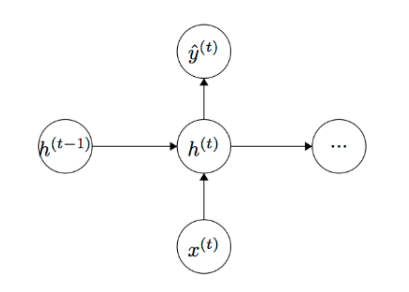
\includegraphics[width = 0.4\textwidth]{chap-05/05-RNN.png}
\caption{RNN单元的输入输出结构}
\label{05-RNN}
\end{figure}

上一节所述的window-based模型在很长一段时间内是主流的语言模型。然而,随着2015年RNN-based模型的兴起,后者已经逐渐取代前者成为主流。当然,长江后浪推前浪,在2019年学术界的兴趣已经转向Attention/Transformer-based模型了。

RNN-based模型的最大特点是对上下文信息的扩充。Window-based模型只能考虑有限大小的上下文,然而RNN-based模型具有记忆性,使用的上下文信息是该句在这个词之前的所有部分\footnote{如果是双向RNN,则上下文是这个单词的所有前后文,包括本句的所有信息。},相比window-based模型具有更大的信息量,所以理论上更能够判断正确。

\begin{figure}[!htbp]
\centering
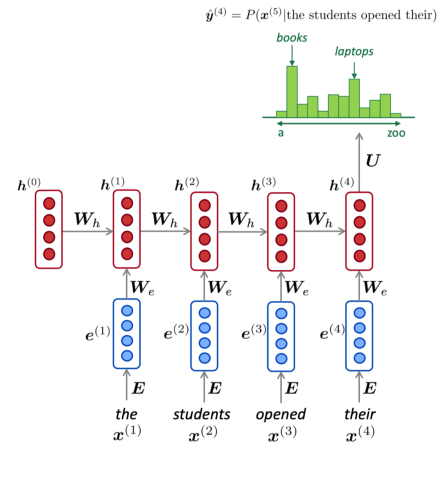
\includegraphics[width = 0.5\textwidth]{chap-05/05-prediction.png}
\caption{RNN可以用于文本生成。}
\label{05-prediction}
\end{figure}

RNN模型经常使用交叉熵和困惑度作为评价指标。对上述概念,\cite{05-tj}讲的很详细。

\subsection{RNN语言模型的特点 \\ Advantages, Disadvantages and Applications of RNNs}

\textbf{优点}

\begin{itemize}
    \item 可以处理变长输入,且模型体量不随输入序列长度增加而增加。RNN对变长的适应性是天然的,不需要做额外的调整,因而在相关问题(比如NLP问题)中一直很受重视。
    \item 具有记忆,可以认为当前词语是基于全部前文决定的。这一点也是RNN相对window-based模型的显著优点。
    \item 所有的输出都通过一组相同的参数计算而得,可以认为预测过程具有普遍性。
\end{itemize}

\textbf{缺点}

\begin{itemize}
    \item 并行程度低,不方便计算。这个问题没法解决,Attention在2017年问世之后逐渐取代RNN也和并行计算方面的因素有关。
    \item 短期记忆问题:因为梯度消失等问题,RNN的记忆性不够,过于靠前的前文对当前词语的判断已经影响不大。\ref{05-solution-vanish}介绍了一些对策。
\end{itemize}

\textbf{内存占用}

运行一层RNN所需的内存量与语料库中的单词数以及句子中的单词数成正比,前者决定了输入One-Hot向量的维数,后者决定了内存中保存向量的个数。另外,内存中还需要保存两对$W, b$系数矩阵。

\subsection{梯度爆炸和梯度消失的对策 \\ Solution to the Exploding and Vanishing Gradients}
\label{05-solution-vanish}

\textbf{梯度爆炸}

梯度爆炸的典型对策是梯度修剪,即当梯度值大于上限阈值时,用一个上限值代替之。

这个方法很朴素,但很有效。如图\ref{05-wall}所示,当在一个如图所示的误差面上训练时,误差本来在平稳地下降(实线箭头),但突然遇到一个梯度极高的地方(高误差壁,High Error Wall),导致这一步梯度极大,导致当前位置的移动到一个极远的位置(实线大箭头),影响下降进度。利用梯度修剪可以让当前位置的移动没有那么远(虚线大箭头),在图中可以继续平稳下降(虚线小箭头)。


\begin{figure}[!htbp]
\centering
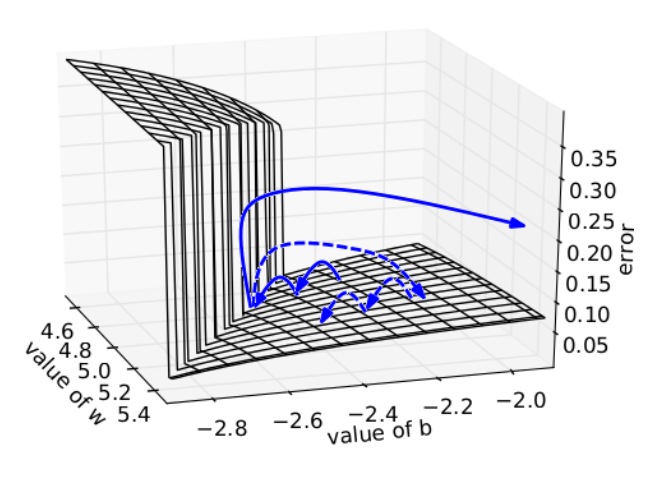
\includegraphics[width = 0.8\textwidth]{chap-05/05-wall.png}
\caption{梯度修剪缓解梯度爆炸问题的一个实证。}
\label{05-wall}
\end{figure}

\textbf{梯度消失}

梯度消失比梯度爆炸更需要控制,因为梯度爆炸会导致数据超过数据范围而报错,而梯度消失会使梯度数值降为0,在这种状况下,我们无法确定当前位置对前文是完全没有依赖,还是有依赖但因为距离太远,梯度已经消失。

梯度消失具有如下对策:

\begin{itemize}
    \item 系数矩阵的初始化不再随机,而是谨慎选取一个恰当位置;
    \item 使用ReLU作为激活函数:因为ReLU的导数不是0就是1,不存在导数$<<1$的状态,因而不会在反向传播的导数值相乘过程中出现梯度消失。
\end{itemize}

随着RNN各种变体的提出,无论是针对单元改进(LSTM),针对结构改进(双向、多层RNN网络)还是在思想上的改进(Encoder-Decoder),都在一定程度上解决了RNN网络短期记忆的问题,梯度爆炸和梯度消失对模型的影响已经逐渐成为历史。

\subsection{基于RNN的机器翻译 \\ Application: RNN Translation Model}

机器翻译领域的传统方法是统计机器翻译,但在深度学习出现之后,神经机器翻译已经体现出巨大的优势。
统计机器翻译(Statistical Machine Translation, SMT)的模型都把翻译分为很多阶段,每个阶段使用不同的方法和模型,整体非常复杂;而神经机器翻译(Neural Machine Translation, NMT)实现了机器翻译的端到端模型,模型简洁,效果突出。
NMT目前的workline主要有三个分支:基于CNN,基于RNN和基于Attention,目前似乎最后一者最火。我们在此主要介绍一些经典的和RNN相关的工作。

最简单的基于RNN的机器翻译模型通过一张图就能说清。如图\ref{05-rnn-nmt}所示。先前的时间阶段输入源语言句子,在源语言句子输入结束后,模型陆续生成目标语言的翻译。
图中在翻译过程中的输入是先前输出的翻译结果,这样能给翻译提供更多的信息。实际上输入其他向量也是可以的,有理由即可,效果另说。

\begin{figure}[!htbp]
\centering
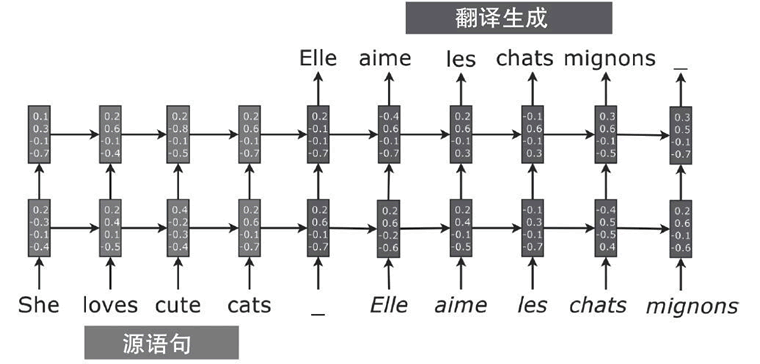
\includegraphics[width=0.8\textwidth]{chap-05/05-rnn-nmt.png}
\caption{最简单的基于RNN的机器翻译模型}
\label{05-rnn-nmt}
\end{figure}

对于这个简陋的模型,实际应用中又有如下改进:

\begin{itemize}
    \item 解码阶段和译码阶段的RNN单元使用不同的权重矩阵;
    \item 把上一个时段的预测输出$\hat{y}$也加入RNN单元的输入;
    \item 使用双向/多层RNN;
    \item 翻转输入序列(但不翻转输出序列)。
\end{itemize}

这些想法都很自然,提出的时候也有背书,而且也都取得了良好的结果。
% \end{multicols}

\section{章节附录}

\subsection{维数灾难 \\ Curse of Dimensionality}
\label{curse}

维数灾难指模型随着数据维数增大而出现问题,无法正常发挥作用的情况。

维数灾难的原理

维数灾难的实例

% 维度灾难
% 我们主要谈自然语言中的维数灾难,从理论和分类上谈,多举例子
% 理论 https://www.cnblogs.com/dingz/p/9029395.html
% 机器学习中的位数灾难 https://blog.csdn.net/qq_39521554/article/details/80653712
% 提到的Bengio论文 https://blog.csdn.net/hx14301009/article/details/80345449

\section*{章节未尽之处}

维数灾难待补

梯度爆炸和梯度消失的理论详解待充实,应该提炼出来放附录

RNN一套待补,其中原来讲义的图特别好,建议借鉴

\begin{thebibliography}{本章节参考文献\&阅读材料}
\bibitem[notes05]{05-this_notes} \url{https://web.stanford.edu/class/cs224n/readings/cs224n-2019-notes05-LM_RNN.pdf}
\bibitem[lecture06]{05-this_slides} \url{https://web.stanford.edu/class/cs224n/slides/cs224n-2019-lecture06-rnnlm.pdf}
\bibitem[lecture07]{05-this_slides2} \url{https://web.stanford.edu/class/cs224n/slides/cs224n-2019-lecture07-fancy-rnn.pdf}
\bibitem[On Chomsky and the Two Cultures of Statistical Learning]{05-stat-fail} \url{http://norvig.com/chomsky.html}
\bibitem[A Neural Probabilistic Language Model]{05-bengio03} \url{http://www.jmlr.org/papers/volume3/bengio03a/bengio03a.pdf}
\bibitem[Word2Vec in gensim]{05-w2v} \url{https://radimrehurek.com/gensim/models/word2vec.html}
\bibitem[Word2Vec CBOW and Skip-Gram]{05-w2v-model} Efficient Estimation of Word Representations in Vector Space, Tomas Mikolov et al, \url{https://arxiv.org/abs/1301.3781}
\bibitem[Word2Vec Optimization]{05-w2v-opti} Distributed Representations of Words and Phrases and their Compositionality, Tomas Mikolov et al, \url{https://arxiv.org/abs/1310.4546}
\bibitem[统计自然语言处理]{05-tj} 统计自然语言处理(第2版),宗成庆,ISBN: 9787302165989,引用2.2.5, 2.2.6, 5.2的内容,这三节分别介绍了交叉熵的定义、困惑度的定义和两者在语言模型中的应用,言简意赅。
\bibitem[统计自然语言处理]{05-tj-qk} 统计自然语言处理(第2版),宗成庆,ISBN: 9787302165989,引用5.1的内容.
\bibitem[计算语言学导论]{05-js} 计算语言学导论,翁富良,王野翊,ISBN: 7500420803
\end{thebibliography}


